\section{Examples}

In this section we introduce and describe some examples of our library usage.
We show thet combinators are expressive enouth for realistic queryes and allows to create generic queryes easely.

\subsection{More complicated example}

Let's form a complex query for our city graph. 
Let us capture one city, let's say city $a$. 
Now having a city graph and captured vertex we would like to know all paths such if as $i$ city from begining of our path we visit country $X$ then as $i$ city from end of our path we visit country $X$ too. 
And also the middle city in our path is our captured city $a$.
In a terms of combinators we can define our path as shown on fig.~\ref{fig:pathQuery}.
Here \lstinline{reduceAsOr} is a function which transforms a list of queries to one query which is formed by reducing given list with \lstinline{|} combinator.
The \lstinline{pathPart} query recursively defines a path of our way.
Also, \lstinline{middleCity} is a vertex query which parses our captured city $a$ and \lstinline{roadTo} query parses a \emph{roadTo} edge.

\begin{figure}[h]
\begin{lstlisting}
val countriesList = List("X", "Y")
val path = 
  (reduceAsOr(countriesList.map(pathPart)) | 
    middleCity)
def pathPart(country: String) =
  syn(city(country) ~ roadTo ~ path ~ 
    roadTo ~ city(country))

val middleCity = V(_.value() == "a")
val roadTo = E(_.value() == "road_to")
def city(country: String) =
  V(_.country == country)
\end{lstlisting}
\caption{Path query}
\label{fig:pathQuery}
\end{figure}


The most exciting feature of our library is that queries can be used as first-class values which means greater generalization and composition. 
The function \lstinline{reduceAsOr} presented in fig~\ref{fig:reduceAsOr} is a !!!!!! WTF!!!!

\begin{figure}[h]
\begin{lstlisting}
def reduceAsOr(xs: List[Nonterminal]) = 
  xs match {
    case x :: Nil     => x
    case x :: y :: xs => 
      syn(xs.foldLeft(x | y)(_ | _))
  }
\end{lstlisting}
\caption{Combinators implementation}
\label{fig:reduceAsOr}
\end{figure}

Now we would like, to get from our query only \lstinline{city} combinator result. 
For that purpose let us modify it to make return result. 
In our library we have a \lstinline{^} and \lstinline{&} functions for that. 
Then we will have definition of our combinators as presented in fig.~\ref{fig:fixedAtor}.

\begin{figure}[h]
\begin{lstlisting}
val middleCity = 
  syn(V(_.value() == "a") ^^) & (List(_))
def pathPart(country: String) = syn(
  (city(country) ~ roadTo ~ 
    path ~ roadTo ~ city(country) & {
      case a ~ (b: List[_]) ~ Entity => 
        a +: b :+ c })
\end{lstlisting}
\caption{Fixed combinators}
\label{fig:fixedAtor}
\end{figure}

Now we execute our query. It is evidente that for the graph presented on fig.~\ref{fig:graph} we can get only three paths which satisfies given criteria:
\begin{itemize}
\item single-vertex path $a$;
\item $b \rightarrow a \rightarrow d$
\item $c \rightarrow b \rightarrow a \rightarrow d \rightarrow e$
\end{itemize}

A simplified SPPF for this query is presented in Fig.~\ref{fig:sppf}: rounded rectangles represent nonterminals and other rectangles represent productions. 
Every rectangle contains a nonterminal name or a production rule, as well as start and end nodes of the path in the input graph derived from the corresponding rectangle. 
Gray rectangles are start nonterminals.

\begin{figure}[h]
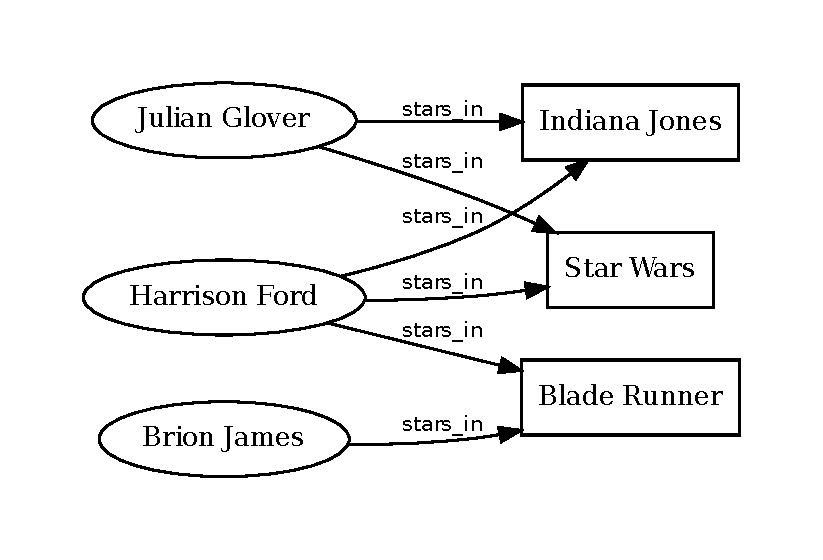
\includegraphics[width=0.45\textwidth]{graph}
\caption{Example Input Graph of Roads}
\label{fig:graph}
\end{figure}


\subsection{Same Generation Query}

Yet another example of first order functions usage is generaligation of classical same generation query which is one of basyc context-free path queries.
One of application of such quries is hierarchy analysing in RDF storages~\cite{RDF}.
Let suppose that we have RDF graphs with two pairs of relation (each pair is relation and its revers): (\emph{subClassOf}; $\text{\emph{subClassOf}}^{-1}$) and (\emph{type}; $\text{\emph{type}}^{-1}$).
We want to evaluate two queries which detect all pairs of nodes which are connected by path derivable in grammars $G_1$~(Fig.~\ref{grammarQ1}) and $G_2$ respectively~(Fig.~\ref{grammarQ2}). 


\begin{figure}[ht]
   \centering
   \[
\begin{array}{rl}
   0: & S \rightarrow \text{\textit{subClassOf}}^{-1} \ S \ \text{\textit{subClassOf}} \\ 
   1: & S \rightarrow \text{\textit{type}}^{-1} \ S \ \text{\textit{type}} \\ 
   2: & S \rightarrow \text{\textit{subClassOf}}^{-1} \ \text{\textit{subClassOf}} \\ 
   3: & S \rightarrow \text{\textit{type}}^{-1} \ \text{\textit{type}} \\ 
\end{array}
\]
   \caption{Contex-free grammar $G_1$ for query 1}
   \label{grammarQ1}
   \end{figure}

\begin{figure}[h]
   \centering
   \[
\begin{array}{rl}
   0: & S \rightarrow B \ \text{\textit{subClassOf}} \\ 
   0: & S \rightarrow \text{\textit{subClassOf}} \\ 
   1: & B \rightarrow \text{\textit{subClassOf}}^{-1} \ B \ \text{\textit{subClassOf}} \\
   2: & B \rightarrow \text{\textit{subClassOf}}^{-1} \ \text{\textit{subClassOf}} \\ 
\end{array}
\]
   \caption{Context-free grammar $G_2$ for query 2}
   \label{grammarQ2}        
   \end{figure}

   Of course, these queryes can be written in Meerkat easely because it supports context-free queryes: code is presented in Fig.~\ref{fig:query1Meerkat} and Fig.~\ref{fig:query2Meerkat}.

\begin{figure}[h]
\begin{lstlisting}
val query1: Nonterminal = syn(
   "subclassof-1" ~ query1.? ~ "subclassof" |
   "type-1" ~ query1.? ~ "type")
\end{lstlisting}
\caption{The same generation query (Query 1) in Meerkat}
\label{fig:query1Meerkat}
\end{figure}


\begin{figure}[h]
\begin{lstlisting}
val S = syn(
  "subclassof-1" ~ S ~ "subclassof")
val query2 = syn(S ~"subclassof")
\end{lstlisting}
\caption{Query 2 grammar}
\label{fig:query2Meerkat}
\end{figure}

As you can see, grammars and code representations for these two quries looks pretty similar.
May we avoid code duplication and generalize them? 
Yes, we can and not only for these two queries.
The function \lstinline{sameGen} presented in Fig~\ref{fig:gen} is a generalization of the same generation query and is independent of the environment such as the input graph structure or other parsers.
It can be used for the creation of other queries, including the one presented in Fig~\ref{fig:query1Meerkat}: it is the result of the application of \lstinline{sameGen} to the appropriate relations (which can be treated as opening and closing brackets).
Another application of the \lstinline{sameGen} is a Query 2, which can be founded in Fig.~\ref{fig:query2Gen}.


\begin{figure}[h]
\begin{lstlisting}
def sameGen(brs) =
  bs.map { case (lbr, rbr) => 
             lbr ~ syn(sameGen(bs).?) ~ rbr } 
  match {
    case x :: Nil => syn(x)
    case x :: y :: xs => 
      syn(xs.foldLeft(x | y)(_ | _))
  }
\end{lstlisting}
\caption{Generic function for the same generations query}
\label{fig:gen}
\end{figure}


\begin{figure}[h]
\begin{lstlisting}
val query1 = syn(sameGen(List(
    ("subclassof-1", "subclassof"),
    ("type-1", "type"))))
\end{lstlisting}
\caption{Query 1 as an application of \lstinline{sameGen}}
\label{fig:query1Gen}
\end{figure}


\begin{figure}[h]
\begin{lstlisting}
val query2 = syn(
  sameGen(List(("subclassof-1", "subclassof"))) ~
   "subclassof")
\end{lstlisting}
\caption{Query 2 as an application of \lstinline{sameGen}}
\label{fig:query2Gen}
\end{figure}


We show that parser combinators provide a simple and safe way to creation of generic queries.
By using this ability, it may be possible to create a library of \ ``standard templates'' for most popular generic queryes like same generatoin query or for domain specific queryes (for example, for specific static code analysis problem).


\subsection{Classical Movies Queries}

!!!!!!!!!!!!!!!!!!!!!!!!!!!!!!!

!!!!!!!!!!!!!!!!!!!!!!!!!!!!!!!

!!!!!!!!!!!!!!!!!!!!!!!!!!!!!!!

!!!!!!!!!!!!!!!!!!!!!!!!!!!!!!!